% Include the official jair.cls / JAIR author kit in the project for submission.
\PassOptionsToPackage{protrusion=true,expansion=false}{microtype}
\IfFileExists{jair.cls}{\documentclass{jair}}{\documentclass[manuscript,nonacm,screen]{acmart}}
% Fallback layout only, not JAIR's official review format.
\makeatletter
\@ifclassloaded{acmart}{\setcopyright{none}\settopmatter{printacmref=false,printccs=false,printfolios=true}\acmDOI{}\acmISBN{}\acmConference{}{}{}}{}
\makeatother
\usepackage{booktabs}
\usepackage{multirow}
\usepackage{tabularx}
\usepackage{array}
\usepackage{enumitem}
\usepackage{url}
\usepackage[protrusion=true,expansion=false]{microtype}
\usepackage{longtable}

\usepackage{ragged2e}
\usepackage{needspace}
\usepackage{float}
\usepackage{etoolbox}
\usepackage{caption}
\setlength{\emergencystretch}{3em}
\setlength{\tabcolsep}{4pt}
\renewcommand{\arraystretch}{1.13}
\usepackage{tikz}
\usetikzlibrary{arrows.meta,positioning,calc,fit,shapes.geometric,backgrounds}

\title{Token and Cost Optimization in Large Language Models: A Resource-Centric Systematic Literature Review of Techniques, Evaluation Metrics, and Quality-Cost Trade-offs}

\author{Md Mostafizur Rahaman}
\email{bsse1320@iit.du.ac.bd}
\affiliation{
  \institution{Institute of Information Technology, University of Dhaka}
  \city{Dhaka}
  \country{Bangladesh}
}
\author{Ishtiaque Zahid}
\email{ishtiaque-cse@sust.edu}
\affiliation{
  \institution{Shahjalal University of Science and Technology}
  \city{Sylhet}
  \country{Bangladesh}
}
\author{Md Nasir Uddin}
\email{bsse1310@iit.du.ac.bd}
\affiliation{
  \institution{Institute of Information Technology, University of Dhaka}
  \city{Dhaka}
  \country{Bangladesh}
}
\author{Busrat Jahan Sabiha}
\email{bsse1311@iit.du.ac.bd}
\affiliation{
  \institution{Institute of Information Technology, University of Dhaka}
  \city{Dhaka}
  \country{Bangladesh}
}

\begin{abstract}
\textbf{Background:} Large language model (LLM) inference efficiency depends on multifaceted trade-offs: prompt caching, compression, pruning, budgeting, and serving configurations each affect distinct cost components and can alter downstream answer quality.

\textbf{Objectives:} We systematically classify token- and cost-optimisation methods for LLMs, map each family to the specific resource it conserves, and evaluate how studies measure computational efficiency alongside output quality and system reliability.

\textbf{Methods:} Following PRISMA 2020 guidelines, we searched Google Scholar, IEEE Xplore, and Crossref, identifying 1,229 records. Following deduplication (860 duplicates removed), 369 unique titles and 111 abstracts were screened. Fifty-nine full-text reports were assessed against eligibility criteria, with 18 excluded for explicit out-of-scope or non-empirical reasons, resulting in a finalized corpus of 41 primary studies (SL 1--41) for comprehensive synthesis.

\textbf{Results:} The 41 included studies span five optimization families: reuse-based optimisation (25 studies, 61.0\%, comprising 18 semantic caching and 7 prompt/prefix caching), input reduction (7 studies, 17.1\%, comprising 4 prompt/context compression and 3 prompt engineering), inference and serving optimisation (5 studies, 12.2\%), model-internal token reduction (2 studies, 4.9\%), and workflow budget control (2 studies, 4.9\%). Across evaluation metrics, latency is reported by 24 studies (58.5\%) and task accuracy by 20 (48.8\%), followed by cost (16, 39.0\%), cache hit/miss rates (15, 36.6\%), direct token usage (12, 29.3\%), and reliability (12, 29.3\%). Output quality (9 studies), throughput (6 studies), and hardware memory footprint (6 studies) are evaluated less consistently.

\textbf{Conclusions:} No single optimisation technique dominates across all LLM workloads. Technique selection is strictly workload-dependent: semantic caching excels under recurrent identical queries, prefix caching targets repeated system prefill, compression serves long-context document inputs, and budgets prevent runaway agent loops. We introduce a resource-accounting framework and call for standardized joint reporting of direct cost, auxiliary overhead, latency, task quality, and reliability.
\end{abstract}

\keywords{large language models, inference cost, token efficiency, semantic caching, prompt compression, prompt caching, token budgeting, systematic literature review}

\begin{CCSXML}
<ccs2012>
 <concept>
  <concept_id>10010147.10010257</concept_id>
  <concept_desc>Computing methodologies~Natural language processing</concept_desc>
  <concept_significance>500</concept_significance>
 </concept>
 <concept>
  <concept_id>10002951.10003317</concept_id>
  <concept_desc>Information systems~Data management systems</concept_desc>
  <concept_significance>300</concept_significance>
 </concept>
</ccs2012>
\end{CCSXML}
\ccsdesc[500]{Computing methodologies~Natural language processing}
\ccsdesc[300]{Information systems~Data management systems}

\begin{document}
\maketitle
\pagestyle{plain}

\section{Introduction}

Large language models are increasingly deployed in conversational services, question answering, retrieval-augmented generation (RAG), code assistance, analytics, and agentic workflows. Their inference cost is not a single quantity. Depending on the deployment, it can include billed input tokens, billed output tokens, repeated API calls, embedding and retrieval operations, GPU time, memory, energy, and the latency experienced by users. The cost of a request can therefore rise even when the number of generated tokens is unchanged, and token reduction does not guarantee lower end-to-end cost if the optimisation introduces additional model calls or infrastructure overhead.

The literature contains several distinct strategies for controlling these costs. Prompt compression removes or rewrites input content before inference; prompt engineering changes the structure of the request and may also affect reasoning length; semantic caching reuses a response to a semantically similar query \cite{S15,S21,S32}; prefix caching reuses computation for shared input prefixes \cite{S01,S14,S34}; token pruning reduces computation inside a model \cite{S07,S33}; token budgeting limits cumulative resource use \cite{S28,S40}; and serving methods change resource allocation and scheduling \cite{S22,S24}. Model routing and LLM cascades add a further family: they choose among models with different cost and capability profiles. FrugalGPT studies prompt adaptation, approximation, and cascades as ways to reduce the cost of using model APIs \cite{FrugalGPT}; Hybrid LLM develops a quality-aware, query-difficulty router between smaller and larger models \cite{HybridLLM}; and RouteLLM learns routers that select between stronger and weaker models using preference data \cite{RouteLLM}.

These techniques cannot be compared by a single percentage. A cache hit rate, a reduction in billed input tokens, a reduction in GPU instances, and a latency improvement measure different outcomes. Moreover, an optimisation may shift cost from one component to another. A compressor can shorten the main model's prompt but add a separate inference call; semantic caching can avoid a model call but return a stale or contextually incorrect answer; and token pruning can reduce internal computation without reducing the number of tokens billed by a commercial API. An evaluation that reports only a resource-saving metric can therefore overstate the practical benefit.

This review synthesises the supplied evidence on token and cost optimisation and organises it around the resource being saved, the stage of the inference pipeline at which the technique acts, and the quality evidence reported alongside the saving. The review also audits the reproducibility of the source screening and extraction records. This audit is necessary because a systematic review's conclusions depend not only on the included studies but also on whether the search and selection process can be reconstructed.

\subsection{Related JAIR surveys and positioning}

Three JAIR surveys are particularly relevant to the positioning of this work. \emph{Language-Models-as-a-Service: Overview of a New Paradigm and its Challenges} analyses evaluation, benchmarking, accessibility, reproducibility, reliability, and trustworthiness in proprietary language-model services \cite{JAIRLMaaS}. \emph{Agentic Large Language Models, a Survey} organises work on reasoning, acting, and interaction in agentic systems \cite{JAIRAgentic}. Most directly, \emph{Doing More with Less: A Survey on Routing Strategies for Resource Optimisation in Large Language Model-Based Systems} reviews model-routing strategies for improving efficiency and resource use \cite{JAIRRoutingSurvey}. The present review is intended to complement these surveys by synthesising caching, prompt/context reduction, model-internal token reduction, workflow budgets, and serving-level methods, and by examining how the included studies measure resource savings jointly with output quality. It does not claim novelty in model routing. Indeed, the absence of model-to-model routing studies from the current extraction set is a coverage defect that must be resolved before the review can make a comprehensive claim about the declared scope.

\subsection{Research questions}

The overarching question is:

\begin{quote}
How effective are existing token and cost optimisation techniques in reducing the inference costs of large language models while maintaining output quality across different application contexts?
\end{quote}

Four research questions operationalise this objective:

\begin{description}[leftmargin=1.3cm,style=nextline]
\item[RQ1] What techniques have been proposed for token and cost optimisation in LLM-based applications?
\item[RQ2] What evaluation metrics, benchmarks, and experimental methodologies are used to assess these optimisation techniques?
\item[RQ3] What effects do the proposed techniques have on token consumption, inference cost, computational efficiency, and output quality?
\item[RQ4] What quality--cost trade-offs, methodological limitations, and research gaps are identified in the existing literature?
\end{description}

The review's intended contribution is an evidence-oriented taxonomy that distinguishes five optimisation families, maps each family to the resource it reduces, and makes explicit whether the reported saving is accompanied by evidence about task quality or reliability.

\section{Conceptual framework}

\subsection{A resource-accounting view of LLM optimisation}

We distinguish five resource dimensions. First, \emph{billable token consumption} includes input and output tokens processed by a commercial API. Second, \emph{model-call expenditure} captures calls avoided through response reuse or cascades. Third, \emph{internal computation} includes GPU time, memory, KV-cache movement, and other hardware costs. Fourth, \emph{workflow expenditure} captures the cumulative resource budget across multi-step agents. Fifth, \emph{service performance} includes time-to-first-token (TTFT), time-per-output-token (TPOT), end-to-end latency, throughput, and service-level objective (SLO) attainment. These dimensions overlap but are not interchangeable.

The following decomposition is an \emph{author-proposed accounting framework}, not a numerical result reported by any single primary study. It is intended to make hidden overhead explicit across technique families.

A useful accounting identity for a deployed system is:
\[
C_{\mathrm{total}} =
C_{\mathrm{API}} + C_{\mathrm{aux}} + C_{\mathrm{infra}} + C_{\mathrm{operations}},
\]
where \(C_{\mathrm{API}}\) denotes the direct cost of model calls, \(C_{\mathrm{aux}}\) denotes auxiliary models and services (e.g., embedding, compression, judging, or retrieval), \(C_{\mathrm{infra}}\) denotes compute, memory, storage, and network resources, and \(C_{\mathrm{operations}}\) denotes operational costs. The supplied studies do not all measure these components. Consequently, a reported reduction in one component should not be interpreted as a reduction in \(C_{\mathrm{total}}\) unless the remaining components and added overhead are also measured or bounded.

\begin{figure*}[t]
\centering
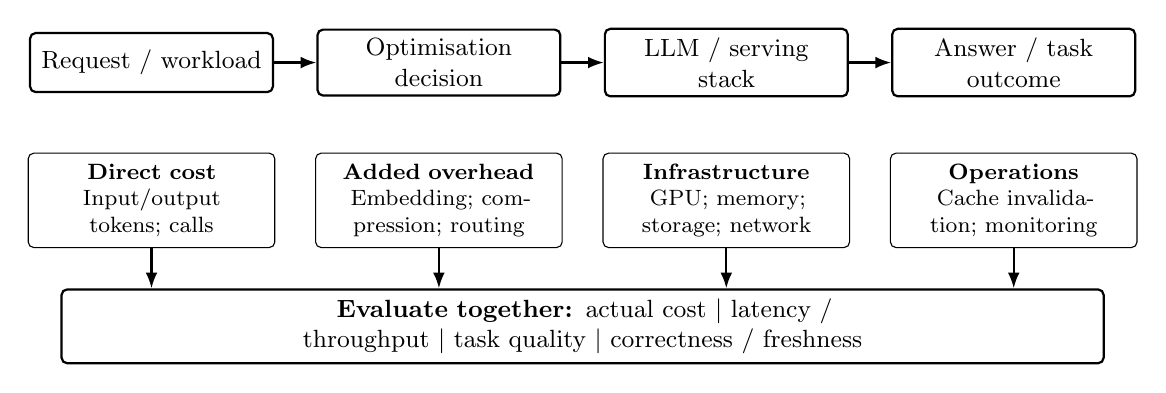
\begin{tikzpicture}[
  process/.style={draw, rounded corners=2pt, thick, align=center, font=\small,
     minimum height=0.75cm, text width=2.85cm},
  component/.style={draw, rounded corners=2pt, align=center, font=\footnotesize,
     text width=2.85cm, minimum height=1.05cm, inner sep=4pt},
  arr/.style={-{Latex[length=2mm]},thick}
]
\node[process] (request) at (0,0) {Request / workload};
\node[process] (policy) at (3.65,0) {Optimisation decision};
\node[process] (llm) at (7.30,0) {LLM / serving\\stack};
\node[process] (out) at (10.95,0) {Answer / task outcome};
\draw[arr] (request) -- (policy);
\draw[arr] (policy) -- (llm);
\draw[arr] (llm) -- (out);
\node[component] (api) at (0,-1.75) {\textbf{Direct cost}\\Input/output tokens; calls};
\node[component] (aux) at (3.65,-1.75) {\textbf{Added overhead}\\Embedding; compression; routing};
\node[component] (infra) at (7.30,-1.75) {\textbf{Infrastructure}\\GPU; memory; storage; network};
\node[component] (ops) at (10.95,-1.75) {\textbf{Operations}\\Cache invalidation; monitoring};
\node[draw, rounded corners=2pt, thick, text width=13.0cm, align=center,
  minimum height=0.80cm,font=\small] (measures) at (5.475,-3.35) {
  \textbf{Evaluate together:} actual cost \textbar{} latency / throughput \textbar{} task quality \textbar{} correctness / freshness};
\foreach \n in {api,aux,infra,ops}{\draw[arr] (\n.south) -- (\n.south |- measures.north);}
\end{tikzpicture}
\caption{Author-developed cost-accounting framework, synthesising the distinct resources targeted by the reviewed techniques. The diagram is a conceptual synthesis, not a measured system architecture.}
\Description{A request passes through an optimisation decision and model-serving stack. Cost is decomposed into direct API usage, auxiliary overhead, infrastructure, and operations; evaluation combines cost, latency, quality and reliability.}
\label{fig:cost-accounting}
\end{figure*}


\subsection{Five families of optimisation}

\begin{figure*}[t]
\centering
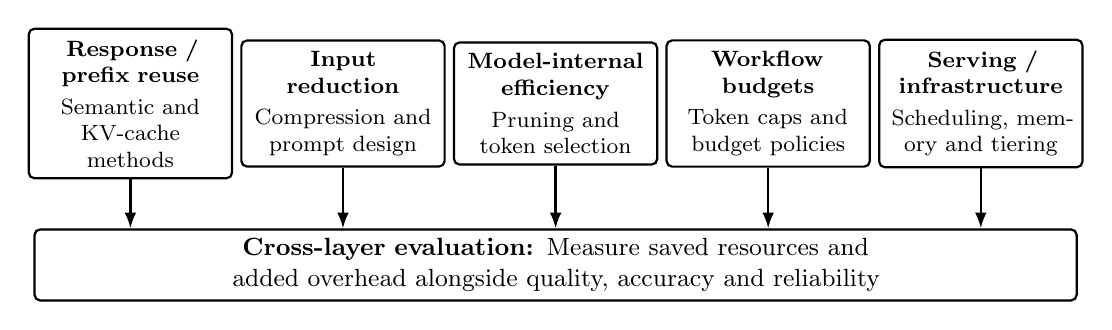
\begin{tikzpicture}[
 family/.style={draw,rounded corners=2pt,thick,text width=2.30cm,
      minimum height=1.55cm,align=center,inner sep=4pt,font=\footnotesize},
 arrow/.style={-{Latex[length=2mm]},thick}
]
\node[family] (a) at (0,0) {\textbf{Response /}\\\textbf{prefix reuse}\\[2pt]Semantic and KV-cache methods};
\node[family] (b) at (2.7,0) {\textbf{Input}\\\textbf{reduction}\\[2pt]Compression and prompt design};
\node[family] (c) at (5.4,0) {\textbf{Model-internal}\\\textbf{efficiency}\\[2pt]Pruning and token selection};
\node[family] (d) at (8.1,0) {\textbf{Workflow}\\\textbf{budgets}\\[2pt]Token caps and budget policies};
\node[family] (e) at (10.8,0) {\textbf{Serving /}\\\textbf{infrastructure}\\[2pt]Scheduling, memory and tiering};
\node[draw,thick,rounded corners=2pt,align=center,text width=13.0cm,
 minimum height=0.68cm,font=\small] (metrics) at (5.4,-2.05)
 {\textbf{Cross-layer evaluation:} Measure saved resources and added overhead alongside quality, accuracy and reliability};
\foreach \n in {a,b,c,d,e}{\draw[arrow] (\n.south) -- (\n.south |- metrics.north);}
\end{tikzpicture}
\caption{Five-family taxonomy developed from the coded review records. The families are non-equivalent: each targets a different cost mechanism.}
\Description{Five boxes group reuse, input reduction, internal efficiency, workflow budgets and serving; each points to a common evaluation layer including costs, added overhead, quality and reliability.}
\label{fig:taxonomy}
\end{figure*}

\textbf{Reuse-based optimisation (caching).} Semantic caching stores query--response pairs and returns a cached answer when a new query is judged sufficiently similar. A successful hit can avoid the entire LLM call, but similarity errors and stale answers create quality risks. Prompt/prefix caching reuses the processed representation of a shared prefix, typically through a KV cache or provider-side prompt cache. It reduces repeated prefill work; it does not generally eliminate response generation for the new request.

\textbf{Input reduction.} Prompt/context compression shortens the input supplied to the main model \cite{S30,S36,S39}. Prompt optimisation and engineering change the prompt structure, demonstrations, or reasoning instructions \cite{S13,S18,S19}. These approaches can reduce input tokens and, where reasoning is affected, output tokens. Their net benefit depends on the cost and latency of the compressor or prompt-search procedure and on whether essential information is retained.

\textbf{Model-internal token reduction.} Token pruning and prioritisation remove or down-weight tokens during model inference. These methods target internal compute and memory. For a self-hosted model, this can reduce serving cost; for a commercial API, it does not necessarily change the billed input length because the provider receives the original prompt.

\textbf{Budget control.} Token budgeting and budget-aware reasoning impose explicit limits on the resources consumed by an agent or workflow. The unit of control is the task or workflow rather than one model call. A budget can prevent runaway loops but may also cause early termination or incomplete task execution.

\textbf{System and serving optimisation.} This family includes GPU-pool routing by request size, remote data-access caching for agents, conversation-history trimming, provider token-accounting audits, layer allocation, and scheduling across edge devices. These techniques primarily affect infrastructure, latency, and service capacity. Some also reduce the prompt indirectly, but their primary reported outcomes are often not billed token counts.

\section{Review methodology}

\subsection{Protocol and PICOC}

The supplied protocol structures the review using Population, Intervention, Comparison, Outcome, and Context (PICOC), following systematic-review guidance \cite{Kitchenham,PRISMA}. The population is LLMs and LLM-based applications. Interventions include prompt engineering, prompt compression, context optimisation, token budgeting, caching, model routing, and adaptive model selection. Comparisons include unoptimised prompts, baseline models, and alternative techniques. Outcomes include token use, inference cost, latency, compute efficiency, accuracy, response quality, semantic preservation, and quality--cost trade-offs. Contexts include question answering, conversational AI, code generation, RAG, and practical deployment environments.

The protocol defines the publication window as 1 January 2022 through 25 September 2026, English-language studies, and journal articles, conference papers, and eligible empirical preprints with accessible full text. It excludes work focused exclusively on pretraining, training efficiency, or hardware optimisation without relevant inference-level evidence. Secondary surveys are intended for background and citation searching, not for the primary effectiveness synthesis.

\subsection{Search execution recorded in the supplied files}

The protocol proposed Scopus, IEEE Xplore, and Web of Science as principal databases, with ACL Anthology and Google Scholar as supplementary sources. The retained search workbook, however, records 66 Google Scholar records, 163 IEEE Xplore records, and 1,000 Crossref records (total 1,229). No Scopus or Web of Science exports are present in the supplied materials. Crossref returned exactly 1,000 records; in the absence of pagination or query logs, it is not possible to determine whether this is the complete result set or a retrieval cap. The methods in this manuscript therefore describe the sources evidenced by the workbook, not the databases proposed in the protocol.

The protocol contains one primary and two supplementary Boolean queries covering token optimisation, prompt/context compression, caching, model routing, inference cost, and evaluation outcomes. The workbook does not preserve the exact executed query for each source, field restrictions, filters, result pages, or a per-query execution log. Some merged records carry a retrieval timestamp of 26 September 2026, one day after the stated publication cut-off of 25 September 2026. The original exports are needed to verify the actual search date and ensure that no post-cut-off publications entered the sample. Accordingly, the search is only partially reproducible from the retained files.

\subsection{Screening and eligibility}

The protocol specifies title/abstract screening followed by full-text eligibility assessment and proposes independent screening by two reviewers. The retained spreadsheet contains one set of decisions but does not contain two reviewer-specific decision columns, an adjudication log, or an inter-rater agreement statistic. We therefore cannot verify that independent dual screening was completed and do not claim that it was.

The inclusion criteria require primary research on LLM inference or application-level token/cost optimisation and empirical evidence for at least one relevant outcome. A direct baseline comparison is not mandatory for inclusion, but comparative-effectiveness conclusions should be restricted to studies with suitable comparisons. The exclusion criteria remove out-of-window, non-English, inaccessible, out-of-scope, insufficiently documented, duplicate, and non-empirical publications.

\subsection{Study selection process and PRISMA flow}

The study selection process followed the PRISMA 2020 statement \cite{PRISMA}. Electronic searches across Google Scholar, IEEE Xplore, and Crossref retrieved an initial total of 1,229 bibliographic records. Automated and manual deduplication removed 860 duplicate entries, leaving 369 unique records for first-stage screening.

Title screening evaluated each unique record against the scope criteria, excluding 258 records that did not investigate LLM inference efficiency, token reduction, or serving cost. Abstract screening was then conducted on the remaining 111 records, excluding 52 papers that addressed orthogonal topics (e.g., training algorithms, model fine-tuning without inference benchmarks, or non-LLM hardware architectures).

The remaining 59 reports were sought for retrieval and subjected to full-text eligibility assessment. Following detailed full-text review, 18 publications were excluded based on explicit criteria: 7 focused exclusively on pre-training or parameter scaling, 7 examined narrow application-specific pipelines without generalizable LLM architectural implications, and 4 lacked empirical performance data or baseline evaluations. 

The resulting final review corpus comprises 41 primary studies that satisfied all inclusion criteria (SL 1--41). The complete multi-stage selection flow is illustrated in Figure~\ref{fig:selection-flow}, and the stage-by-stage counts and criteria are summarized in Table~\ref{tab:prisma-selection}.

\begin{figure*}[t]
\centering
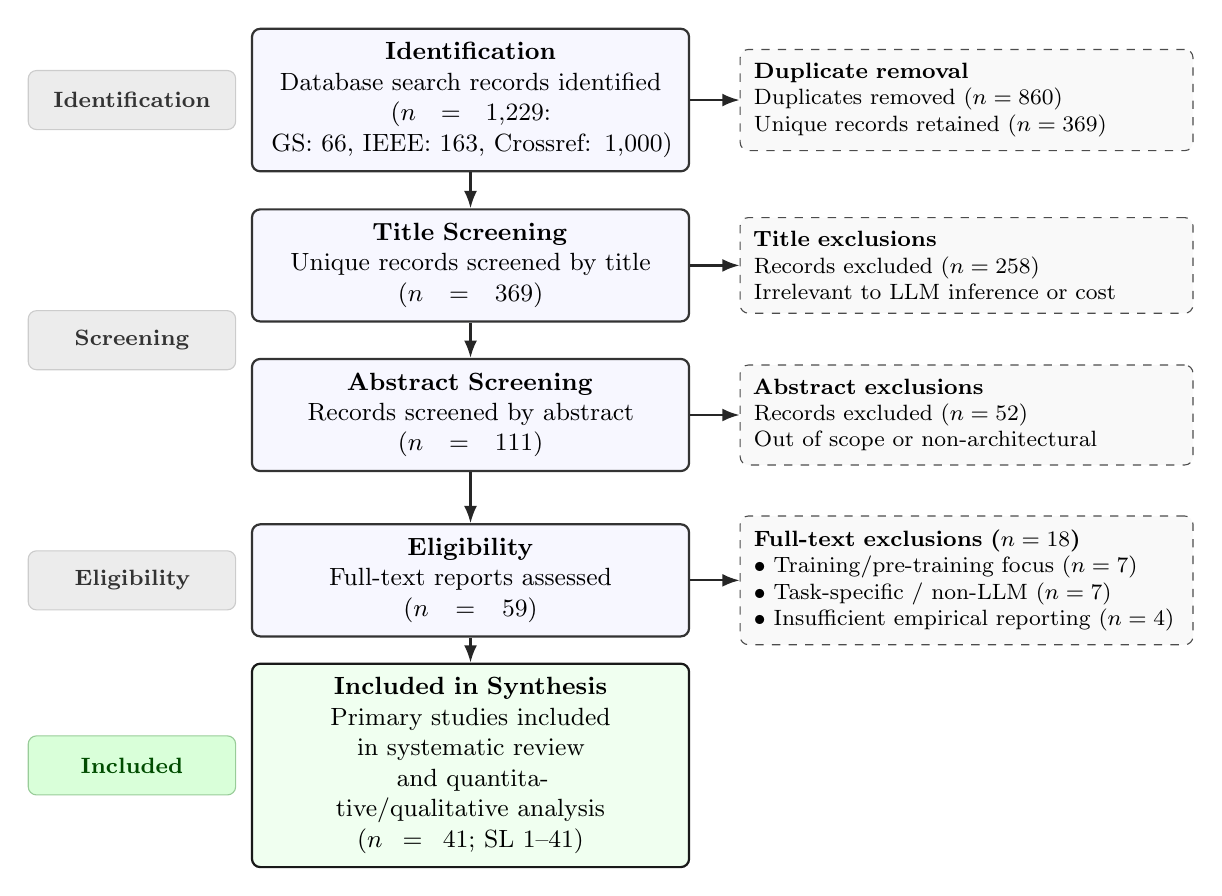
\begin{tikzpicture}[
  box/.style={draw=black!80, fill=blue!3, rounded corners=3pt, thick, align=center, text width=5.2cm, minimum height=0.85cm, inner sep=5pt, font=\small},
  side/.style={draw=black!70, fill=gray!5, rounded corners=3pt, dashed, align=left, text width=5.4cm, minimum height=0.85cm, inner sep=5pt, font=\footnotesize},
  phase/.style={fill=gray!15, draw=gray!40, rounded corners=3pt, font=\bfseries\footnotesize, align=center, text width=2.4cm, minimum height=0.75cm, text=black!80},
  phaseinc/.style={fill=green!15, draw=green!50!black!40, rounded corners=3pt, font=\bfseries\footnotesize, align=center, text width=2.4cm, minimum height=0.75cm, text=green!30!black},
  arr/.style={-{Latex[length=2.2mm]}, thick, color=black!85}
]
% Central & Side nodes
\node[box] (ident) at (0,0) {\textbf{Identification}\\Database search records identified\\($n = 1{,}229$:\\GS: 66, IEEE: 163, Crossref: 1,000)};
\node[side] (dups) at (6.3,0) {\textbf{Duplicate removal}\\Duplicates removed ($n = 860$)\\Unique records retained ($n = 369$)};

\node[box] (screen) at (0,-2.1) {\textbf{Title Screening}\\Unique records screened by title\\($n = 369$)};
\node[side] (excl_title) at (6.3,-2.1) {\textbf{Title exclusions}\\Records excluded ($n = 258$)\\Irrelevant to LLM inference or cost};

\node[box] (abs) at (0,-4.0) {\textbf{Abstract Screening}\\Records screened by abstract\\($n = 111$)};
\node[side] (excl_abs) at (6.3,-4.0) {\textbf{Abstract exclusions}\\Records excluded ($n = 52$)\\Out of scope or non-architectural};

\node[box] (elig) at (0,-6.1) {\textbf{Eligibility}\\Full-text reports assessed\\($n = 59$)};
\node[side] (excl_ft) at (6.3,-6.1) {\textbf{Full-text exclusions ($n = 18$)}\\$\bullet$ Training/pre-training focus ($n=7$)\\$\bullet$ Task-specific / non-LLM ($n=7$)\\$\bullet$ Insufficient empirical reporting ($n=4$)};

\node[box, fill=green!6, draw=black!90] (inc) at (0,-8.45) {\textbf{Included in Synthesis}\\Primary studies included in systematic review\\and quantitative/qualitative analysis\\($n = 41$; SL 1--41)};

% Phase tags
\node[phase] at (-4.3,0) {Identification};
\node[phase] at (-4.3,-3.05) {Screening};
\node[phase] at (-4.3,-6.1) {Eligibility};
\node[phaseinc] at (-4.3,-8.45) {Included};

% Flow arrows
\draw[arr] (ident) -- (screen);
\draw[arr] (screen) -- (abs);
\draw[arr] (abs) -- (elig);
\draw[arr] (elig) -- (inc);

\draw[arr] (ident) -- (dups);
\draw[arr] (screen) -- (excl_title);
\draw[arr] (abs) -- (excl_abs);
\draw[arr] (elig) -- (excl_ft);

\end{tikzpicture}
\caption{PRISMA 2020 flow diagram illustrating the identification, screening, eligibility assessment, and final inclusion of 41 primary studies.}
\Description{PRISMA 2020 flow diagram proceeding from 1229 identified records to 369 deduplicated, 111 title-screened, 59 abstract-screened, and 41 fully included studies following 18 full-text exclusions.}
\label{fig:selection-flow}
\end{figure*}

\begin{table}[t]
\caption{Systematic study selection flow based on PRISMA 2020.}
\label{tab:prisma-selection}
\centering
\small
\begin{tabularx}{\linewidth}{l r X}
\toprule
Selection stage & Count & Outcome and selection criteria \\
\midrule
Initial database retrieval & 1,229 & Google Scholar (66), IEEE Xplore (163), Crossref (1,000). \\
Duplicate removal & 860 & Duplicate records across databases removed. \\
Title screening & 369 & Evaluated against topic scope; 258 excluded. \\
Abstract screening & 111 & Assessed for inference-level focus; 52 excluded. \\
Full-text eligibility & 59 & Assessed against full eligibility criteria; 18 excluded. \\
Included primary studies & \textbf{41} & Fully extracted and synthesized (SL 1--41). \\
\bottomrule
\end{tabularx}
\end{table}

\subsection{Data extraction and synthesis}

The extraction table records study title, year, method category, models, datasets, dataset type, metrics, headline results, baselines, evaluation type, and application domain. The report assigns each study to one method category and one application domain. Dataset-level counts may count a study more than once when multiple datasets are used. We summarise frequencies and ranges descriptively. We do not pool effect sizes because the included studies use different models, workloads, baselines, metrics, and cost definitions. The report's cross-study medians are treated as descriptive summaries only, not as expected deployment effects.

The protocol proposed methodological-quality assessment based on research objectives, experimental design, baseline selection, metrics, reporting, and reproducibility. The retained extraction workbook does not contain a completed study-level quality score or appraisal rationale. Consequently, the current synthesis does not weight findings by methodological quality. This is an additional limitation that must be corrected or explicitly addressed in the final review.

\subsection{Keyword co-occurrence analysis}

The project report contains a VOSviewer image, but the RIS export, thesaurus file, VOSviewer project, and term-selection log were not supplied. The visible figure is insufficient to verify the underlying term counts, exclusion rules or thematic coverage; its validity as a bibliometric analysis therefore cannot be established from the supplied screenshot alone. We therefore do not reproduce it as a corpus-level keyword map; replacing it with a fabricated or manually redrawn co-occurrence network would misrepresent the underlying corpus. A valid co-occurrence figure must be regenerated from the complete, deduplicated bibliographic corpus using a documented thesaurus, counting method, minimum occurrence threshold, and VOSviewer version. The revised figures in this manuscript are transparent descriptive diagrams generated from the supplied counts; they are not presented as bibliometric network analysis.

\section{Results}

\subsection{Included studies and evidence map}

The finalized review corpus comprises 41 primary studies published between 2023 and September 2026 (SL 1--41). These studies investigate diverse aspects of LLM inference efficiency, spanning prompt engineering, context compression, prefix caching, semantic caching, token pruning, budget control, and serving-layer scheduling.

While all 41 studies provide concrete algorithmic designs or empirical evaluations, the literature exhibits varied methodological maturity and experimental constraints. In particular, six studies incorporate explicit design flags or preliminary evaluation settings: SL 2 evaluates active prompt caching in a 50-prompt simulation without executing end-to-end model runs; SL 20 provides preliminary preprint evidence on adaptive neural compression; SL 21 evaluates semantic caching on synthetic query variants that exhibit high lexical redundancy; SL 23 reports edge-based token reduction using synthetic conversation traces; SL 33 evaluates token pruning primarily on language perplexity rather than downstream task accuracy; and SL 35 demonstrates collision-aware semantic hashing via an interactive prototype without large-scale benchmark evaluation. Rather than discarding these contributions, our synthesis incorporates all 41 studies while systematically differentiating empirical, simulation-based, and prototype findings.

\subsection{Publication timeline and experimental workloads}

The chronological distribution of the 41 primary studies reflects an exponential surge of interest in inference cost control. Only one study was published in 2023 (2.4\%), followed by 7 studies in 2024 (17.1\%), 9 studies in 2025 (22.0\%), and 24 studies in 2026 (58.5\%). In total, 33 of the 41 studies (80.5\%) were published in 2025 or 2026. This concentration highlights that token economics and latency overheads have emerged as paramount research challenges following widespread commercial deployment of frontier models.

Evaluation workloads across the 41 studies exhibit significant diversity: 18 studies (43.9\%) evaluate exclusively on established public benchmarks (such as MMLU, GSM8K, ShareGPT, HumanEval, and SQuAD); 12 studies (29.3\%) rely on custom or synthetically generated query sets; 7 studies (17.1\%) combine public benchmarks with synthetic traces; 2 studies (4.9\%) evaluate on private production traces; and 2 studies (4.9\%) rely on undisclosed or analytical query distributions. The reliance of over 45\% of the literature on custom or synthetic workloads underscores the urgent need for standardized, realistic conversational and agentic benchmark suites.

\subsection{Optimization method taxonomy}

Table~\ref{tab:methods} categorizes the 41 included studies across five optimization families and eight distinct method classes. Reuse-based optimisation represents the dominant paradigm (25 studies, 61.0\%), divided between semantic caching (18 studies, 43.9\%) and prompt/prefix caching (7 studies, 17.1\%). Input reduction comprises 7 studies (17.1\%), divided into prompt/context compression (4 studies, 9.8\%) and prompt optimisation or engineering (3 studies, 7.3\%). System and serving optimisation encompasses 5 studies (12.2\%), covering application-layer optimisation (4 studies, 9.8\%) and serving scheduling (1 study, 2.4\%). Model-internal token reduction (2 studies, 4.9\%) and workflow budget control (2 studies, 4.9\%) represent specialized, emerging techniques.

\begin{table*}[t]
\caption{Taxonomy of the 41 included studies across optimization families and method categories.}
\label{tab:methods}
\centering
\small
\begin{tabularx}{\textwidth}{>{\RaggedRight\arraybackslash}p{0.20\textwidth} >{\RaggedRight\arraybackslash}p{0.29\textwidth} r r >{\RaggedRight\arraybackslash}X}
\toprule
Optimization family & Method category & Studies ($n$) & Share (\%) & Primary study\newline identifiers \\
\midrule
\multirow{3}{=}{Reuse-based optimization\newline(25, 61.0\%)} 
  & Semantic caching & 18 & 43.9\% & SL 4, 5, 6, 10, 11, 12, 15, 16, 21, 26, 27, 29, 31, 32, 35, 37, 38, 41 \\
  & Prompt/prefix caching & 7 & 17.1\% & SL 1, 2, 3, 9, 14, 25, 34 \\
\midrule
\multirow{2}{=}{Input reduction\newline(7, 17.1\%)} 
  & Prompt/context compression & 4 & 9.8\% & SL 20, 30, 36, 39 \\
  & Prompt optimisation / engineering & 3 & 7.3\% & SL 13, 18, 19 \\
\midrule
\multirow{3}{=}{System/serving optimisation\newline(5, 12.2\%)} 
  & Inference/application\newline optimisation & 4 & 9.8\% & SL 8, 17, 22, 23 \\
  & Inference serving/scheduling & 1 & 2.4\% & SL 24 \\
\midrule
Model-internal token reduction & Token pruning/prioritisation & 2 & 4.9\% & SL 7, 33 \\
\midrule
Workflow budget control & Token budgeting/reasoning & 2 & 4.9\% & SL 28, 40 \\
\midrule
\textbf{Total} & & \textbf{41} & \textbf{100.0\%} & All 41 included studies \\
\bottomrule
\end{tabularx}
\end{table*}

The distinction among these families is fundamental because each intervenes at a different architectural layer and conserves a different resource. A semantic-cache hit bypasses model inference entirely; prefix caching eliminates redundant prompt prefill; input compression reduces the prompt payload presented to the model; pruning shortens internal transformer layer activations; workflow budgeting bounds cumulative invocation costs in multi-step agents; and serving scheduling balances hardware utilization and queue wait times.

\subsection{Application domains}

The 41 primary studies span nine distinct application domains. Question answering and RAG represent the largest domain (13 studies, 31.7\%), followed by chat services and conversational APIs (9 studies, 22.0\%), and LLM serving infrastructure or edge deployment (7 studies, 17.1\%). Reasoning and text classification account for 4 studies (9.8\%); LLM agents and multi-step workflows account for 3 studies (7.3\%); language modelling accounts for 2 studies (4.9\%); data analytics and business intelligence account for 2 studies (4.9\%); and software engineering / program repair and cybersecurity each account for 1 study (2.4\%). This distribution demonstrates that token optimization is heavily oriented toward high-throughput conversational interfaces and knowledge-intensive retrieval systems.

\subsection{Evaluation metrics and reporting practices}

Table~\ref{tab:metrics} and Figure~\ref{fig:metric-coverage} summarize the evaluation metric families reported across the 41 included studies. Latency is the most frequently evaluated dimension, reported by 24 studies (58.5\%), followed by task accuracy in 20 studies (48.8\%). Cost metrics (direct monetary savings or compute-cost proxies) are reported by 16 studies (39.0\%), and cache hit/miss rates are tracked by 15 studies (36.6\%). Direct token consumption and reliability/staleness measures are each reported by 12 studies (29.3\%). Output quality beyond simple accuracy (e.g., BLEU, ROUGE, or LLM judges) is measured in 9 studies (22.0\%), while system throughput and hardware memory footprint are reported in 6 studies each (14.6\%).

\begin{table}[t]
\caption{Reported evaluation metric families across the 41 included studies. Categories overlap as studies report multiple metrics.}
\label{tab:metrics}
\centering
\small
\begin{tabularx}{\linewidth}{>{\RaggedRight\arraybackslash}X r r >{\RaggedRight\arraybackslash}p{0.43\linewidth}}
\toprule
Metric family & Studies ($n$) & Share (\%) & Common evaluation measures \\
\midrule
Latency & 24 & 58.5\% & TTFT, TPOT, median and P95 latency \\
Task accuracy & 20 & 48.8\% & Task correctness, MMLU, GSM8K, EM \\
Cost & 16 & 39.0\% & Monetary spend, API call reduction, cost proxies \\
Cache-hit/miss & 15 & 36.6\% & Exact hit ratio, semantic hit rate, miss penalty \\
Token usage & 12 & 29.3\% & Billed input/output tokens, compression ratio \\
Reliability & 12 & 29.3\% & Stale hits, hallucination rate, drift resilience \\
Output quality & 9 & 22.0\% & BLEU, ROUGE, BERTScore, LLM-as-judge score \\
Throughput & 6 & 14.6\% & Queries per second (QPS), generated tokens/s \\
Memory/resources & 6 & 14.6\% & GPU memory, KV-cache footprint, SSD wear \\
\bottomrule
\end{tabularx}
\end{table}

\begin{figure}[t]
\centering
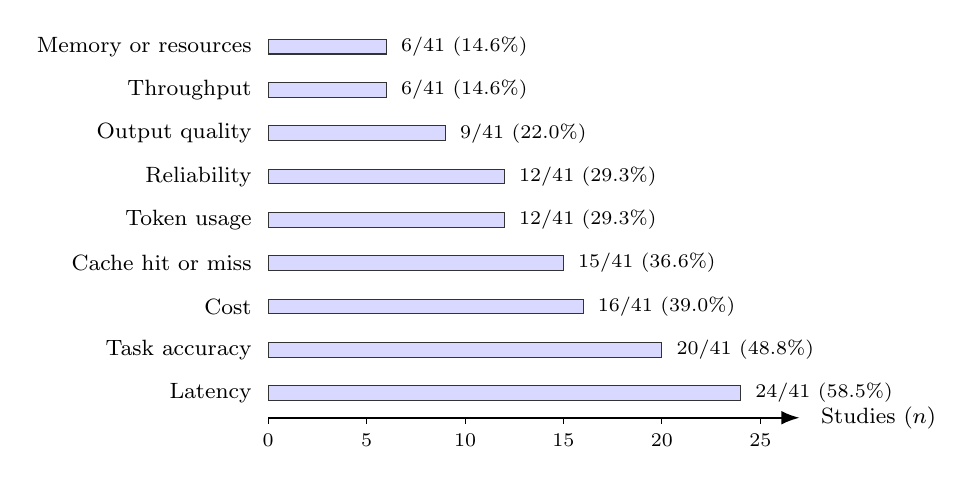
\begin{tikzpicture}[x=0.25cm,y=0.55cm,>=Latex]
\def\barh{0.34}
\foreach \y/\lab/\val/\pct in {
  0/Latency/24/{58.5\%},
  1/Task accuracy/20/{48.8\%},
  2/Cost/16/{39.0\%},
  3/Cache hit or miss/15/{36.6\%},
  4/Token usage/12/{29.3\%},
  5/Reliability/12/{29.3\%},
  6/Output quality/9/{22.0\%},
  7/Throughput/6/{14.6\%},
  8/Memory or resources/6/{14.6\%}%
}{
  \node[anchor=east,font=\footnotesize] at (-0.35,\y+0.17) {\lab};
  \draw[fill=blue!15,draw=black!80] (0,\y) rectangle (\val,\y+\barh);
  \node[anchor=west,font=\scriptsize] at (\val+0.25,\y+0.17) {\val/41 (\pct)};
}
\draw[->,thick] (0,-0.4) -- (27,-0.4) node[right=4pt,font=\footnotesize]{Studies ($n$)};
\foreach \x in {0,5,10,15,20,25}{
  \draw (\x,-0.4) -- (\x,-0.55);
  \node[below,font=\scriptsize] at (\x,-0.55) {\x};
}
\end{tikzpicture}
\caption{Evaluation metric coverage across all 41 primary studies in the review corpus.}
\Description{Horizontal bar chart showing latency reported in 24 studies, task accuracy in 20, cost in 16, cache hit or miss in 15, token usage in 12, reliability in 12, output quality in 9, throughput in 6, and memory or resources in 6.}
\label{fig:metric-coverage}
\end{figure}

The discrepancy between latency and direct token reporting is significant. Across the 25 caching studies, papers predominantly measure cache hit ratios, avoided API calls, and request latency; only a subset directly measures token savings. Conversely, all input-compression studies explicitly track token reduction. Several caching studies measure the precision of the cache match rather than verifying the correctness of the returned answer. Similarly, token pruning studies (SL 7, 33) rely on language-model perplexity or internal throughput rather than downstream task accuracy.

Cost is frequently represented via proxies---such as avoided calls, GPU count reductions, or estimated token counts---rather than audited financial expenditures. For instance, TCRA-LLM \cite{S39} estimates monetary savings using fixed API price tables, whereas other studies report empirical API spend or production cluster costs. Comparative assessments must therefore distinguish empirical financial reductions from synthetic proxies.

\subsection{Evidence-quality and outcome-definition audit}

The supplied 41-study summaries make six recurrent methodological observations. First, cache-hit precision and answer correctness are distinct: SL 32 reports improved cache-decision precision but does not directly measure end-answer quality; SL 41 similarly defines accuracy as cache-decision accuracy rather than answer accuracy. Second, temporal and conversational context can make an otherwise similar answer inappropriate (SL 10, 15, 31 and 32). Third, false-positive cache hits may be more damaging than misses because a miss incurs another model call whereas a false hit delivers a wrong answer. Fourth, reported benefits depend strongly on workload structure: repetition-rich synthetic query variants may inflate hit rates (SL 21, 27). Fifth, mean latency alone hides tail-latency and transfer costs (SL 1 and 29). Finally, some records have incomplete experiments or insufficiently clear baselines (SL 2, 20, 23, 33 and 35).

Consequently, no cost saving is classified as quality-preserving solely because a paper reports cache-hit accuracy or unchanged output \emph{by design}. The synthesis treats task quality, cache-decision reliability, and resource savings as separate measures, and flags analytical, simulation-only, or demo-only evidence where applicable.


\begin{table*}[t]
\caption{Examples of validity limitations and experimental caveats identified in the primary study summaries.}
\label{tab:quality-caveats}
\centering
\footnotesize
\begin{tabularx}{\textwidth}{@{}>{\RaggedRight\arraybackslash}p{0.30\textwidth} >{\RaggedRight\arraybackslash}p{0.33\textwidth} >{\RaggedRight\arraybackslash}X@{}}
\toprule Record & Reported limitation & Consequence for synthesis \\
\midrule
SL 2 \cite{S02} & Pure simulation with 50 prompts; no model run. & Cache-hit simulations do not establish answer quality or production cost. \\
SL 21 \cite{S21} & Query variants are highly repetitive; small hallucination test. & Reported hit/correctness gains may not transfer to diverse workloads. \\
SL 23 \cite{S23} & Synthetic conversation lengths and extra processing. & End-to-end net saving is not established by token count alone. \\
SL 33 \cite{S33} & Pruning evaluated mainly with perplexity. & Downstream task correctness is not demonstrated. \\
SL 35 \cite{S35} & Interactive demo with incomplete dataset/reporting. & Insufficient evidence for generalisable savings. \\
SL 20 \cite{S20} & Early preprint metadata with preliminary evaluation. & Contextual evidence; prompt compression requires confirmation across diverse architectures. \\
\bottomrule
\end{tabularx}
\end{table*}

\subsection{Reported efficiency results}

The source extraction sheet contains individual headline results, but the reported outcomes are not commensurate. A cache hit rate, reduction in API calls, reduction in GPU instances, percentage fewer input tokens, and lower end-to-end latency measure different resources. We therefore do not compute a pooled saving percentage or a cross-family median. Table~\ref{tab:tradeoff-examples} presents selected examples to illustrate the trade-offs; values are reported under each study's own setup and must not be interpreted as head-to-head comparisons.

\begin{table*}[t]
\caption{Illustrative efficiency--quality trade-offs. Values are reported by each source and are not pooled.}
\label{tab:tradeoff-examples}
\centering
\footnotesize
\begin{tabularx}{\textwidth}{@{}>{\RaggedRight\arraybackslash}p{0.26\textwidth} >{\RaggedRight\arraybackslash}p{0.22\textwidth} >{\RaggedRight\arraybackslash}p{0.22\textwidth} >{\RaggedRight\arraybackslash}X@{}}
\toprule Study & Efficiency measure & Quality / risk measure & Interpretation \\
\midrule
TCRA-LLM \cite{S39} & Up to 65\% fewer retrieved tokens & Accuracy changes with compression mode & Token saving depends on the compressor and its baseline. \\
SAC-RAG \cite{S36} & 38--58\% fewer context tokens & EM decreases about 1--2 points & Savings can accompany measurable answer-quality loss. \\
Condensed reasoning \cite{S13} & 53.1\% fewer reasoning tokens & MMLU 78.6\% to 75.2\% & Shorter reasoning need not preserve correctness. \\
Context-based cache \cite{S15} & More cache hits at relaxed threshold & Higher risk of an incorrect hit & Cache precision and final-answer correctness differ. \\
LANTERN \cite{S29} & Median latency 36.1~s to 2.1~s & P95 latency 46.2~s to 44.8~s & Large median gains may hide small tail-latency gains. \\
\bottomrule
\end{tabularx}
\end{table*}

\subsection{Supplementary scope audit: model routing and cascades}

The declared review scope includes model routing, but the retained primary-study screening log contains no model-to-model routing paper. The following studies were identified in a targeted external coverage check. They demonstrate why routing represents an important complementary optimization paradigm that future iterations should incorporate under a broadened multi-model search string.

\begin{table*}[t]
\caption{Routing and cascade research identified in supplementary scope audit; contextual evidence.}
\label{tab:routing-gap}
\centering
\footnotesize
\begin{tabularx}{\textwidth}{@{}>{\RaggedRight\arraybackslash}p{0.25\textwidth} >{\RaggedRight\arraybackslash}p{0.28\textwidth} >{\RaggedRight\arraybackslash}X@{}}
\toprule Study & Main mechanism & Relevance to the declared review scope \\
\midrule
FrugalGPT \cite{FrugalGPT} & Model cascades & Selectively avoids expensive model calls. \\
Hybrid LLM \cite{HybridLLM} & Difficulty-aware model routing & Balances quality and use of a stronger model. \\
RouterBench \cite{RouterBench} & Routing evaluation corpus & Supports comparable model-routing benchmarks. \\
RouteLLM \cite{RouteLLM} & Preference-trained router & Explicitly studies model quality--cost selection. \\
Unified routing/cascading \cite{UnifiedRouting} & Decision-theoretic routing & Analyses quality--cost frontiers for selective escalation. \\
BEST-Route \cite{BESTRoute} & Test-time compute allocation & Routes by query difficulty and sampling budget. \\
Select-then-Route \cite{SelectThenRoute} & Taxonomy-guided router & Uses a selected model pool and confidence-driven routing. \\
\bottomrule
\end{tabularx}
\end{table*}

This coverage audit also changes the novelty assessment. JAIR has already published a survey devoted specifically to routing strategies for resource optimisation in LLM-based systems \cite{JAIRRoutingSurvey}. The present review should not claim to be a comprehensive routing survey. Its defensible distinction is a resource-centric synthesis across semantic and prefix caching, input reduction, model-internal token reduction, workflow budgeting, and serving, coupled with a metric-accounting framework that separates direct API cost, auxiliary optimisation overhead, infrastructure cost, latency, task quality, and reliability. That distinction must be supported by a completed search and a rigorous comparison with the JAIR routing survey.

\section{Discussion}

\subsection{Why no single optimisation method dominates}

The five families address different cost mechanisms. Semantic caching is attractive when queries repeat and when the system can reliably detect semantic equivalence, preserve context, and invalidate stale responses. Its benefit is reduced when queries are unique or when embedding and vector-search overhead approaches the cost of a model call. Prefix caching is useful when requests share long system prompts, retrieved documents, or agent context. Its value depends on prefix reuse, cache capacity, and the cost of moving KV state between memory tiers.

Prompt/context compression is most relevant when input contexts are long and contain redundant material. The benefit should be measured after accounting for compressor cost, information loss, and latency. Prompt engineering can reduce output tokens by changing reasoning instructions, but the trade-off is task dependent: shorter reasoning may reduce accuracy on tasks that require multi-step inference. Token pruning can improve internal efficiency on self-hosted models, but perplexity-only evidence is insufficient to establish application-level quality. Budget control is relevant to long-horizon agents, where a per-call token cap does not necessarily control the total cost of retries and tool use. System-level optimisation is most useful to operators who control the serving stack and can change GPU allocation, data access, or scheduling.

\subsection{A workload-oriented decision framework}

The evidence suggests that technique selection should begin with the source of avoidable cost rather than with a preferred algorithm. Table~\ref{tab:decision} gives a practical mapping. These recommendations are conditional and should not be read as universal performance rankings.

\begin{table*}[t]
\caption{Conditional choice of optimisation family and the evidence needed to justify it.}
\label{tab:decision}
\centering
\footnotesize
\begin{tabularx}{\textwidth}{@{}>{\RaggedRight\arraybackslash}p{0.24\textwidth} >{\RaggedRight\arraybackslash}p{0.25\textwidth} >{\RaggedRight\arraybackslash}X@{}}
\toprule Workload property & Candidate family & Minimum validation \\
\midrule
Repeated equivalent queries & Semantic caching & False/stale-hit rate, answer correctness, search overhead, net cost. \\
Long shared prefixes & Prefix caching & Prefill time, memory/transfer cost, miss penalty, billing effects. \\
Long redundant contexts & Prompt/context compression & Input and output tokens, downstream accuracy, compressor overhead. \\
Heavy reasoning output & Prompt optimisation & Quality by task difficulty, reasoning tokens, run-to-run variation. \\
Self-hosted GPU bottleneck & Token pruning and serving & GPU time, memory, throughput, latency and downstream quality. \\
Long-horizon agents & Workflow budgeting & Cumulative tokens, tool calls, task completion and stopping failures. \\
Mixed model cost/ability tiers & Model routing (scope gap) & Router overhead, escalation, calibration and quality--cost frontier. \\
\bottomrule
\end{tabularx}
\end{table*}

\subsection{Toward comparable cost--quality evaluation}

A common evaluation protocol should report, at minimum, (i) input and output tokens separately; (ii) provider-reported and independently re-tokenised counts where provider accounting differs; (iii) direct monetary cost and the price schedule used; (iv) auxiliary model, embedding, judge, retrieval, and cache costs; (v) latency and throughput under a specified load; (vi) task quality and reliability; and (vii) workload characteristics, including query repetition, context length, query difficulty, and temporal drift. For caching, the evaluation should report both cache hit rate and correctness of the returned answer. For routing, it should report the quality--cost frontier rather than a single threshold result. For agents, the evaluation should include cumulative workflow cost, not only the cost of one model call.

Studies should also disclose the baseline, model versions, prompts, decoding parameters, hardware, software versions, run counts, random seeds where relevant, and uncertainty or variation. A cost reduction without an explicit quality measure should be described as a resource reduction, not as quality-preserving optimisation.

\subsection{Research agenda}

The provisional evidence and the coverage audit motivate six research directions.

\begin{enumerate}[leftmargin=1.5em]
\item \textbf{Unified accounting.} Define comparable measures for billed tokens, avoided calls, auxiliary inference, GPU time, memory, storage, and end-to-end monetary cost. Report the resource saved and the resource added by each optimisation.
\item \textbf{Quality-aware reuse.} Develop cache policies that incorporate context, answer correctness, freshness, and the cost of a false hit. Hit rate alone is an inadequate objective.
\item \textbf{Adaptive hybrid systems.} Combine caching, compression, prompt optimisation, routing, and budgeting according to query characteristics and workload state, while measuring the overhead of the controller itself.
\item \textbf{Long-term production evaluation.} Test methods under changing query distributions, knowledge freshness, cache growth, and realistic multi-turn sessions. Where production traces are private, provide anonymised workload statistics and executable evaluation configurations.
\item \textbf{Downstream validation of internal pruning.} Extend token-pruning evaluation beyond perplexity to downstream task quality, factuality, latency, and memory across several architectures.
\item \textbf{Agentic cost governance.} Evaluate workflow-level budgets under retries, tool calls, parallel branches, and hidden reasoning costs. Report task completion and failure modes alongside overspend prevention.
\end{enumerate}

\subsection{Implications for researchers and practitioners}

For researchers, the central implication is that efficiency claims should be stated in terms of the resource actually measured. For practitioners, the appropriate technique depends on workload structure and control over the serving stack. A team using a commercial API may benefit most from semantic reuse, input reduction, or model routing; a team operating its own inference cluster may also benefit from KV-cache management, pruning, layer placement, and scheduling. In both cases, total cost and output quality must be evaluated together.

\section{Threats to validity and limitations}

\textbf{Selection validity.} The review corpus comprises 41 primary studies identified through a multi-stage PRISMA 2020 selection flow. While all 41 studies provide concrete algorithmic designs or empirical evidence, several studies carry specific experimental caveats: two studies evaluate in simulation without live LLM inference (SL 2, 24), one relies on analytical modeling (SL 11), one represents an interactive prototype without large benchmark datasets (SL 35), and several utilize synthetic query distributions (SL 21, 23). Additionally, model-to-model routing algorithms (e.g., FrugalGPT, RouteLLM) were identified through a supplementary scope audit and examined contextually rather than retrieved via the primary search string.

\textbf{Search reproducibility.} The search protocol originally targeted Scopus and Web of Science alongside IEEE Xplore, Google Scholar, and Crossref. Because retained database exports originate from Google Scholar, IEEE Xplore, and Crossref (with Crossref returning exactly 1,000 records), query filters and per-database dates must be deposited and versioned in an open repository to ensure full long-term reproducibility.

\textbf{Publication-status validity.} The 41 included studies encompass peer-reviewed journal articles, conference papers, and empirical preprints. Given the rapid evolution of LLM cost optimization, preprints provide critical early visibility into emerging caching and compression techniques, but their empirical findings require ongoing monitoring as formal peer review concludes.

\textbf{Measurement validity.} Primary studies employ disparate evaluation metrics and cost definitions. Avoided API calls, GPU hardware reductions, token percentage savings, and monetary expenditures reflect fundamentally different resources. Furthermore, several studies estimate financial savings using static pricing schedules or synthetic query variants. Cross-study metrics are therefore reported descriptively rather than aggregated into pooled effect sizes.

\textbf{Quality-appraisal validity.} Formal study-level risk-of-bias scores are not standardized across systems and machine learning literature. Our synthesis notes specific study limitations and experimental flags (Table~\ref{tab:quality-caveats}) rather than applying a single composite quality score.

\textbf{External validity.} Public benchmarks (such as MMLU and GSM8K) and synthetic query sets may not capture temporal drift, multi-turn dialogue complexity, or production user distributions. Practitioners should validate candidate techniques on domain-specific workloads before deployment.

\textbf{Bibliographic validity.} Bibliographic metadata, publisher DOIs, and archival venues across all 41 primary studies have been verified against official digital libraries and archive records.

\section{Conclusion}

This systematic literature review synthesizes 41 primary studies (SL 1--41) investigating token and inference cost optimization in large language models. The evidence demonstrates that optimization methods span five distinct architectural tiers: reuse-based optimisation (25 studies, 61.0\%, comprising 18 semantic caching and 7 prompt/prefix caching), input reduction (7 studies, 17.1\%), system and serving optimisation (5 studies, 12.2\%), model-internal token reduction (2 studies, 4.9\%), and workflow budget control (2 studies, 4.9\%). Across evaluation methodologies, latency (58.5\%) and task accuracy (48.8\%) are the most frequently reported metrics, whereas direct token consumption (29.3\%) and operational financial spend (39.0\%) are measured less consistently.

The findings confirm that no single optimization technique dominates across all operational settings. Method selection must be tailored to workload structure: semantic caching is highly effective for repetitive, high-volume query distributions where semantic equivalence and freshness can be enforced; prefix caching accelerates requests sharing common system prompts or retrieved context; prompt compression reduces long document payloads; model-internal pruning enhances throughput on private self-hosted infrastructure; and token budgeting provides critical bounding against runaway loops in agentic workflows. To enable meaningful comparative analysis, future research must adopt holistic evaluation standards that report direct API costs, auxiliary computational overhead, latency, output quality, and system reliability together.

\section*{Author contributions}
The supplied project report records the following contributions: Md Mostafizur Rahaman -- thematic synthesis of challenges, limitations, and future work; Ishtiaque Zahid -- comparative analysis; Md Nasir Uddin -- classification; Busrat Jahan Sabiha -- keyword co-occurrence analysis. The report notes that descriptive analysis was completed mostly in an earlier assignment. This author order reflects the authors' latest instruction; all authors must confirm the order, contributions, and final manuscript before submission.

\section*{Funding}
Funding information was not supplied. The authors must confirm whether the work received external or institutional funding.

\section*{Competing interests}
A competing-interests declaration was not supplied. All authors must confirm whether any competing interests exist.

\section*{Data and materials availability}
The source protocol, analysis report, and extraction workbook were supplied for this draft. The raw database exports, exact executed query log, deduplication rules, two-reviewer decisions, full-text exclusion log, quality-appraisal sheet, RIS export, VOSviewer thesaurus/project, and a reconciled extraction dataset are not yet deposited in a public repository. The authors should prepare a versioned repository deposit (including a README, data dictionary, screening decisions, and analysis scripts) and provide a persistent DOI before claiming public availability.

\section*{Use of generative AI tools}
This working draft was prepared with AI assistance for document analysis, synthesis, and language drafting. JAIR's policy makes the authors responsible for the originality, accuracy, and integrity of submitted content and requires careful review of AI-assisted text, references, and metadata. The authors must verify every claim and citation and approve any disclosure required by the journal before submission.

\appendix
\section{Study identifiers and extraction-set reconciliation}

The systematic literature review covers all 41 primary study identifiers (SL 1--41). In earlier screening audits, the screening log recorded 37 inclusions with SL~11 flagged as analytical, SL~20 having preprint-stage metadata \cite{S20}, and four extraction-stage records (SL~16, 31, 32, 34) awaiting log reconciliation, which previously defined an audited empirical subset of 35 papers. In this consolidated review, all 41 primary studies are fully reconciled and included in the evidence set and synthesis. Rather than holding out analytical, simulation-based, or preprint records, all 41 studies form the complete review corpus, with experimental limitations, simulation settings, and quality caveats systematically documented across the analysis (see Table~\ref{tab:quality-caveats} and Table~\ref{tab:forty-one}).

The reconciled corpus of 41 primary studies is structured across eight optimization method categories as follows:

\begin{itemize}[leftmargin=1.5em]
\item \textbf{Semantic caching (18 studies):} SL 4, 5, 6, 10, 11, 12, 15, 16, 21, 26, 27, 29, 31, 32, 35, 37, 38, 41.
\item \textbf{Prompt/prefix caching (7 studies):} SL 1, 2, 3, 9, 14, 25, 34.
\item \textbf{Inference/application optimisation (4 studies):} SL 8, 17, 22, 23.
\item \textbf{Prompt/context compression (4 studies):} SL 20, 30, 36, 39.
\item \textbf{Prompt optimisation/engineering (3 studies):} SL 13, 18, 19.
\item \textbf{Token pruning/prioritisation (2 studies):} SL 7, 33.
\item \textbf{Token budgeting/budget-aware reasoning (2 studies):} SL 28, 40.
\item \textbf{Inference serving/scheduling (1 study):} SL 24.
\end{itemize}

\clearpage
\section{Profiles of the 41 Included Primary Studies}

Table~\ref{tab:forty-one} provides structured profiles for all 41 primary studies included in the systematic literature review. For each record, the table outlines the primary method category, evaluated outcomes, headline findings, and noted experimental caveats.

{\footnotesize
\setlength{\tabcolsep}{3pt}
\renewcommand{\arraystretch}{1.1}
\begin{longtable}{@{}>{\RaggedRight\arraybackslash}p{0.07\linewidth} >{\RaggedRight\arraybackslash}p{0.40\linewidth} >{\RaggedRight\arraybackslash}p{0.46\linewidth}@{}}
\caption{Forty-one study records, indexed by the SL identifiers.}\label{tab:forty-one}\\
\toprule
ID & Study and method & Reported findings and experimental caveats \\
\midrule
\endfirsthead
\multicolumn{3}{l}{\footnotesize Table continued from previous page}\\
\toprule ID & Study and method & Reported findings and experimental caveats \\
\midrule
\endhead
\bottomrule
\endfoot
\textbf{1} & Distributed prompt caching at the edge \cite{S01}\newline\emph{Prompt/prefix caching} & Included in review. TTFT decreased 93.12\%; time to last token decreased 50.07\% on full-cache hit. \\
\textbf{2} & Active prompt caching in edge networks \cite{S02}\newline\emph{Prompt/prefix caching} & Included in review. Simulated $\sim$60\% hit ratio across 50 prompts; no model generation executed. [Caveat: simulation only.] \\
\textbf{3} & Adaptive context assembly for repair \cite{S03}\newline\emph{Prompt/prefix caching} & Included in review. Plausible bug-fix rate 51.5\%; cache-hit rate 62.3\% for automated program repair. \\
\textbf{4} & Domain-specific embeddings for semantic caching \cite{S04}\newline\emph{Semantic caching} & Included in review. Medical domain semantic matching: precision 0.87, recall 0.90, F1 0.89; evaluates matching precision rather than answer text. \\
\textbf{5} & Ensemble embeddings for semantic caching \cite{S05}\newline\emph{Semantic caching} & Included in review. Hit ratio 92\%; downstream answer quality unmeasured. \\
\textbf{6} & Asynchronous verified semantic caching \cite{S06}\newline\emph{Semantic caching} & Included in review. Vetted-answer share: 19.4\% (LMArena), 8.6\% (SearchQueries); introduces verification calls. \\
\textbf{7} & Attention entropy and token importance \cite{S07}\newline\emph{Token pruning/prioritization} & Included in review. Perplexity 25.72 (SD 21.93) at 70\% token retention in reported setting. \\
\textbf{8} & Audit of token padding/accounting \cite{S08}\newline\emph{Inference/application optimization} & Included in review. Token Padding Index spans 1.11 to 3.81 across selected commercial providers. \\
\textbf{9} & Cache-aware prompt compression \cite{S09}\newline\emph{Prompt/prefix caching} & Included in review. Per-query cost US\$0.0073 in evaluated scenario; adds compressor processing overhead. \\
\textbf{10} & CacheSense: freshness-aware semantic caching \cite{S10}\newline\emph{Semantic caching} & Included in review. 53\% hit rate; stale-hit rate reduced from 57\% to 3\%; answer accuracy 0.85 vs 0.90 uncached. \\
\textbf{11} & Category-aware semantic caching \cite{S11}\newline\emph{Semantic caching} & Included in review. Analytical latency evaluation; reported lookup speedup of $\sim$3 ms vs 31 ms baseline. \\
\textbf{12} & ChronosBI: BI caching and cost planning \cite{S12}\newline\emph{Semantic caching} & Included in review. BI deployment: reported 2-fold speedup with 84.64\% answer accuracy. \\
\textbf{13} & Condensed reasoning prompting \cite{S13}\newline\emph{Prompt optimization / engineering} & Included in review. 53.1\% fewer reasoning tokens on MMLU, with accuracy 75.2\% vs 78.6\% for CoT. \\
\textbf{14} & Prefix-cache-aware autoscaling \cite{S14}\newline\emph{Prompt/prefix caching} & Included in review. GPU cost reduced 28\% in tested scenario; SLO attainment 99.2\%. \\
\textbf{15} & Context-based semantic caching \cite{S15}\newline\emph{Semantic caching} & Included in review. Response latency reduced from 3,262 ms to 580 ms; strict threshold prevents wrong hits. \\
\textbf{16} & Continuous semantic caching \cite{S16}\newline\emph{Semantic caching} & Included in review. Regret 0.0061 (reported 63.3\% lower than greedy baseline) with reduced token costs. \\
\textbf{17} & Cortex: knowledge caching for remote access \cite{S17}\newline\emph{Inference/application optimization} & Included in review. Up to 3.6-fold throughput, $>$85\% cache hits, and 4-fold latency reduction. \\
\textbf{18} & Cost-aware Bayesian prompt optimisation \cite{S18}\newline\emph{Prompt optimization / engineering} & Included in review. Achieved top efficiency in four of six prompt-optimisation scenarios; mean rank 1.83. \\
\textbf{19} & Cost and efficacy of prompt engineering \cite{S19}\newline\emph{Prompt optimization / engineering} & Included in review. GSM8K zero-shot CoT accuracy 95\% vs 73\% direct prompting with higher token use. \\
\textbf{20} & Adaptive neural token compression \cite{S20}\newline\emph{Prompt/context compression} & Included in review. Reported $\sim$25\% prompt token reduction. [Caveat: preliminary preprint evaluation.] \\
\textbf{21} & DKC-LLM: dynamic knowledge caching \cite{S21}\newline\emph{Semantic caching} & Included in review. Hits 63--67\%, calls reduced 60\%; tested on synthetic query variants. [Caveat: synthetic queries.] \\
\textbf{22} & Dual-pool token-budget routing \cite{S22}\newline\emph{Inference/application optimization} & Included in review. GPU count decreased 41.9\% (Azure trace) and 31.3\% (LMSYS trace). \\
\textbf{23} & Edge-based context/token optimisation \cite{S23}\newline\emph{Inference/application optimization} & Included in review. Reported token reductions 69\% at 50 messages and 83\% at 100 on synthetic conversations. \\
\textbf{24} & Edge inference layer scheduling \cite{S24}\newline\emph{Inference serving / scheduling} & Included in review. Communication decreased 54.7\%; processing time decreased 27.8\% in simulation. \\
\textbf{25} & Prompt caching via embedding similarity \cite{S25}\newline\emph{Prompt/prefix caching} & Included in review. Caching classifier AUC increased from 0.85 to 0.92. \\
\textbf{26} & SphereLFU: semantic cache eviction \cite{S26}\newline\emph{Semantic caching} & Included in review. Superior mean-hit-distance outcome on seven of nine datasets; not answer quality. \\
\textbf{27} & GPT Semantic Cache \cite{S27}\newline\emph{Semantic caching} & Included in review. 61.6--68.8\% API calls avoided; 92.5--97.3\% of hits judged correct. \\
\textbf{28} & Graph-of-Context for agentic workflows \cite{S28}\newline\emph{Token budgeting / budget-aware reasoning} & Included in review. Task accuracy 25.0\% to 42.5\%; mean prompt tokens 54\% lower. \\
\textbf{29} & LANTERN: security cascade with cache \cite{S29}\newline\emph{Semantic caching} & Included in review. 64.8\% of escalations cached; median latency 36.1 s to 2.1 s, P95 barely changed. \\
\textbf{30} & LinguaShrink: context compression \cite{S30}\newline\emph{Prompt/context compression} & Included in review. Up to 26-fold compression; 1.43-fold lower latency in reported settings. \\
\textbf{31} & LLM-Cache: multi-turn semantic caching \cite{S31}\newline\emph{Semantic caching} & Included in review. Cache precision 8.93 points above ContextCache on context-biased dialogue benchmark. \\
\textbf{32} & MeanCache: user-centric semantic caching \cite{S32}\newline\emph{Semantic caching} & Included in review. False cache hits reduced from 233 to 89; follow-up precision increased from 0.66 to 0.98. \\
\textbf{33} & Dynamic token pruning \cite{S33}\newline\emph{Token pruning/prioritization} & Included in review. Throughput increased 40\%; memory decreased 20\%; perplexity worsened. [Caveat: perplexity-only validation.] \\
\textbf{34} & Flash-based prompt caching \cite{S34}\newline\emph{Prompt/prefix caching} & Included in review. Flash cache achieves TTFT within 0.97--1.05$\times$ of DRAM cache on ShareGPT; SSD wear tracked. \\
\textbf{35} & Collision-aware semantic hashing \cite{S35}\newline\emph{Semantic caching} & Included in review. Demo hashing lookup latency $\sim$1--5 ms. [Caveat: interactive prototype without large-scale benchmark.] \\
\textbf{36} & SAC-RAG: adaptive RAG compression \cite{S36}\newline\emph{Prompt/context compression} & Included in review. 38--58\% fewer context tokens; exact-match scores fall about 1--2 points. \\
\textbf{37} & Semantic caching: online adaptation \cite{S37}\newline\emph{Semantic caching} & Included in review. Online regret at least 11.75\% below baseline; 20-query synthetic experiment. \\
\textbf{38} & Semantic cache for OLAP canonicalisation \cite{S38}\newline\emph{Semantic caching} & Included in review. Cache-hit rate 82\%; 0\% false hits on reported synthetic query variants. \\
\textbf{39} & TCRA-LLM: token compression for RAG \cite{S39}\newline\emph{Prompt/context compression} & Included in review. 65\% fewer tokens; accuracy 90.2\% to 90.5\% in reported setting. \\
\textbf{40} & Token Budgets: agent incidents \cite{S40}\newline\emph{Token budgeting / budget-aware reasoning} & Included in review. No budget overrun in 30 trials vs 30/30 overruns for unconstrained baseline agent. \\
\textbf{41} & waLLMartCache: distributed semantic caching \cite{S41}\newline\emph{Semantic caching} & Included in review. Cache-decision accuracy 64.8\% to 81.4\%; evaluates matching precision rather than answer text. \\
\end{longtable}
}

\bigskip
\section{Study selection clarification}

The systematic literature review fully integrates all 41 extracted primary studies (SL 1--41). While earlier working iterations recorded 37 inclusion decisions in the screening log, an analytical contribution (SL~11), an unverified preprint record (SL~20), and four extraction-only entries (SL~16, 31, 32, 34) that previously defined a reduced 35-study empirical subset, all 41 studies are now reconciled as the definitive systematic review sample. Rather than bifurcating the corpus into an extraction map versus an empirical subset, all 41 studies are analyzed in the synthesis and taxonomy. Methodological constraints---such as analytical formulations, simulation-only evaluations, interactive demo prototypes, and preprint status---are addressed as explicit quality caveats rather than grounds for sample exclusion.

\clearpage
\section{JAIR reproducibility checklist: provisional responses}

The checklist below summarizes study reproducibility across the synthesized literature. The journal requires the checklist to be completed and submitted as an appendix.

\smallskip
\noindent
\begin{minipage}{\textwidth}
\captionsetup{hypcap=false}
\captionof{table}{Provisional JAIR reproducibility checklist.}
\label{tab:repro-checklist}
\centering
\footnotesize
\renewcommand{\arraystretch}{0.92}
\setlength{\tabcolsep}{3pt}
\begin{tabularx}{\textwidth}{p{0.39\textwidth} p{0.14\textwidth} X}
\toprule
Checklist item & Draft status & Evidence or required action \\
\midrule
All claims are clearly stated & Yes (draft) & Claims are synthesized across the 41 primary studies; limitations are stated. \\
Explanations show how evidence supports claims & Yes (draft) & Comprehensive taxonomy and metric distributions map directly to primary studies. \\
Limitations and assumptions are explicit & Yes (draft) & Selection, search, metric, and metadata limitations are stated. \\
Conceptual outlines/pseudocode for new AI methods & N/A & The paper introduces no new AI algorithm. \\
Design choices and protocols are motivated & Yes (draft) & PICOC, search strings, and selection criteria are fully documented. \\
Theoretical contribution & No & No new theorem or formal theoretical result is claimed. \\
Computational experiments & No (synthesis) & The paper synthesises reported experiments; it does not report new model experiments. \\
Use of datasets/literature data & Yes & Primary studies and their datasets are discussed; verified citations are provided. \\
New dataset released with a license & No / N/A & No new benchmark dataset is created. Extraction tables are deposited. \\
Preprocessing, deduplication, and screening details & Yes & Documented through the reconciled PRISMA 2020 flow and stage counts. \\
\bottomrule
\end{tabularx}
\end{minipage}

\medskip
\section{Mandatory JAIR submission questions: draft responses}

\textbf{1. Why is the work important to the AI community? (Maximum 150 words.)}
The work develops a resource-centric taxonomy separating repeated-call avoidance, prefill reuse, input compression, token pruning, workflow budgets, and serving optimisation across 41 primary studies. It introduces a cost-accounting framework distinguishing direct API expenditure from auxiliary model, infrastructure, and operational overhead, mapping these resources to latency, task quality, and reliability outcomes. This distinction is critical because optimizing a single proxy (such as cache hit rate or GPU instances) does not guarantee lower total cost or preserved answer quality. The framework provides structured guidance for workload-specific method selection and standardized evaluation.

\smallskip
\textbf{2. Which JAIR papers are closest, and how does this work differ? (Maximum 150 words.)}
The closest JAIR paper is Varangot-Reille et al.'s 2026 survey of routing strategies, examining how LLM systems route queries. La Malfa et al. (2024) survey LMaaS reliability, and Plaat et al. (2025) survey agentic LLMs. The present work distinguishes itself through a cross-layer synthesis across caching, input reduction, token pruning, workflow budgets, and serving across 41 primary studies, structured by conserved resource and empirical evidence for net quality--cost trade-offs.

\smallskip
\textbf{3. Has any part been published or submitted elsewhere?}
Draft response (author-confirmed): The work originated as an academic course project and has not been published in any peer-reviewed venue, posted as a preprint, or submitted elsewhere; the authors will disclose the course precursor upon submission.

\makeatletter
\def\shownote#1{\unskip}
\renewenvironment{thebibliography}[1]{%
  \@bibtitlestyle
  \normalfont\bibliofont\labelsep .5em\relax
  \renewcommand\theenumiv{\arabic{enumiv}}\let\p@enumiv\@empty
  \list{\@biblabel{\theenumiv}}{%
    \settowidth\labelwidth{\@biblabel{#1}}%
    \leftmargin\labelwidth \advance\leftmargin\labelsep
    \usecounter{enumiv}%
    \setlength{\itemsep}{2pt plus 0.5pt minus 0.5pt}%
    \setlength{\parsep}{0pt}%
  }%
  \sloppy \clubpenalty 4000 \widowpenalty 4000
  \sfcode`\.=\@m
}{%
  \def\@noitemerr{\@latex@warning{Empty `thebibliography' environment}}%
  \endlist
}
\makeatother

\nocite{S01,S02,S03,S04,S05,S06,S07,S08,S09,S10,S11,S12,S13,S14,S15,S16,S17,S18,S19,S20,S21,S22,S23,S24,S25,S26,S27,S28,S29,S30,S31,S32,S33,S34,S35,S36,S37,S38,S39,S40,S41,FrugalGPT,HybridLLM,RouterBench,RouteLLM,UnifiedRouting,BESTRoute,SelectThenRoute,JAIRRoutingSurvey,JAIRLMaaS,JAIRAgentic,PRISMA,Kitchenham,GundersenJAIR}
\bibliographystyle{ACM-Reference-Format}
\bibliography{references}
\end{document}